\documentclass{beamer}
\usepackage[style=authortitle,backend=bibtex]{biblatex}
\addbibresource{presentation.bib}
\usepackage{media9}

\usepackage[latin1]{inputenc}
\usepackage[justification=centering]{caption}
\usepackage{multicol}
\usepackage{color}
\usepackage{xcolor}
	\definecolor{DarkGreen}{RGB}{0,120,0}
\usepackage{epsfig}
\usetheme{Warsaw}
\usepackage{subcaption}
\usepackage{mwe}
\usepackage{wrapfig}
\usepackage{hyperref}
\usepackage{graphicx}
\usepackage[export]{adjustbox}

\begin{document}


\title[Leading the fight against fake news]{Leading the fight against fake news}

% \author[S. Cidambi, S. Merry, D. Srivastava, G. Vattiato]{Sahana Cidambi \and Stephen Merry \and Duttatrey Srivastava \and Giorgia Vattiato}

\author[S. Cidambi, S. Merry, D. Srivastava, G. Vattiato]
{	\begin{tabular}{ c c }
		Sahana Cidambi & Stephen Merry         \\  
		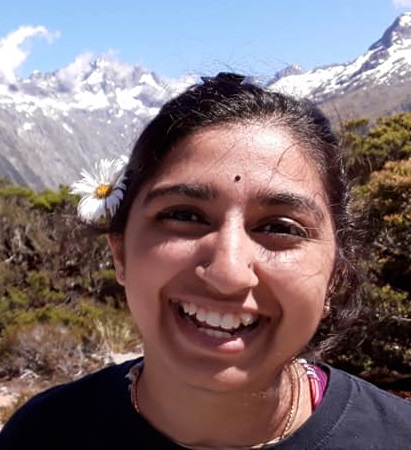
\includegraphics[scale=0.13]{Figures/Sahana.jpg} & 
\includegraphics[scale=0.05]{Figures/Stephen.jpg}  \\
		 & \\
		Duttatrey Srivastava & Giorgia Vattiato        \\  
		
\includegraphics[scale=0.12]{Figures/Dutta.jpg} & 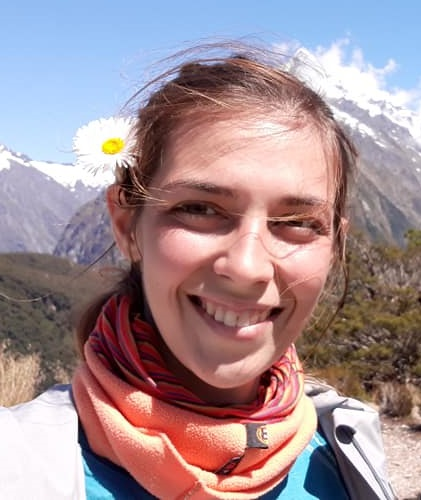
\includegraphics[scale=0.13]{Figures/Giorgia.jpg}    
	\end{tabular}}

\date{}

%%%%%%%%%%%%%%%%%%%%%%%%%%%%%%%%%%%%%%%%

\frame{\titlepage}

%%%%%%%%%%%%%%%%%%%%%%%%%%%%%%%%%%%%%%%%

\begin{frame} \frametitle{Problem Statement}
Fake news
	    \begin{itemize}
			\item Type of yellow journalism
			\item Deliberate disinformation or hoaxes spread via traditional news media
			\item For people such as children and the elderly, spotting fake news is a near impossible task
		\end{itemize}
		\vfill
	\begin{tabular}{ c c }
	
			
\includegraphics[scale=0.3,frame]{Figures/Chemtrails.pdf} & 
\includegraphics[scale=0.3,frame]{Figures/Vaccines.pdf}  \\ \multicolumn{2}{c}{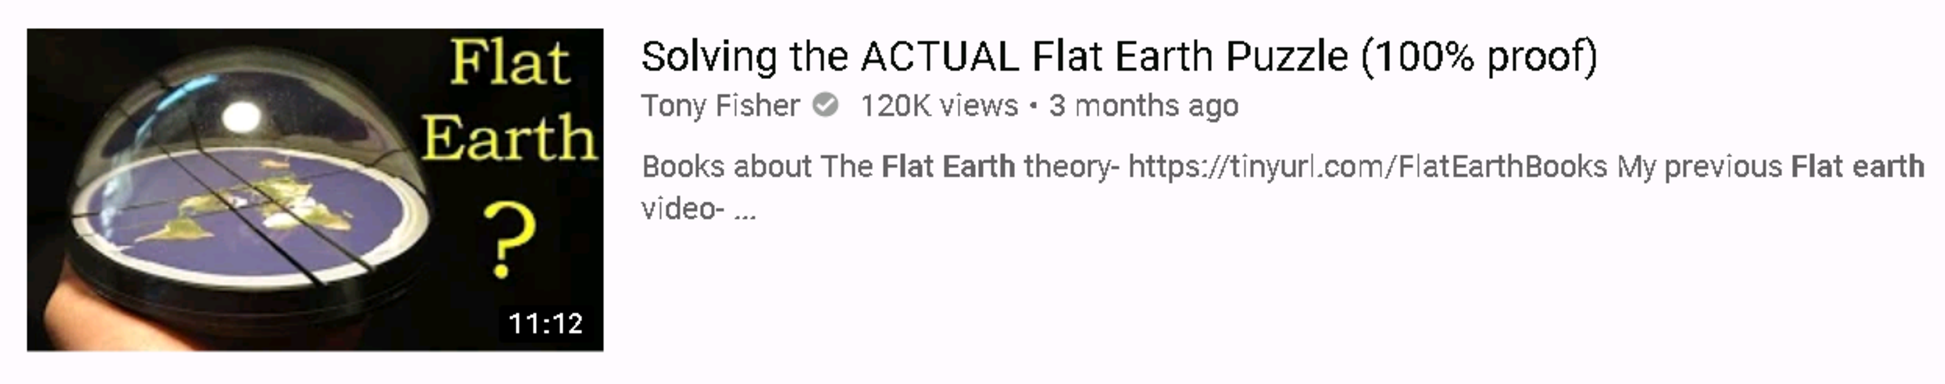
\includegraphics[scale=0.25,frame]{Figures/Flat_earth.pdf}}
	\end{tabular}	
		

% \begin{columns}
% 		\column{0.6\textwidth}
		
		
% 		\column{0.3\textwidth}
% 		\begin{figure}
% 			
\includegraphics[scale=0.3]{Figures/Chemtrails.pdf}
% 		\end{figure}
% 	\end{columns}		
% 	\begin{figure}
% 		\centering
% 		\begin{minipage}{0.5\textwidth}
% 			\centering
% 			
\includegraphics[scale=0.3]{Figures/Vaccines.pdf}
% 		\end{minipage}\hfill
% 		\begin{minipage}{0.5\textwidth}
% 			\centering
% 			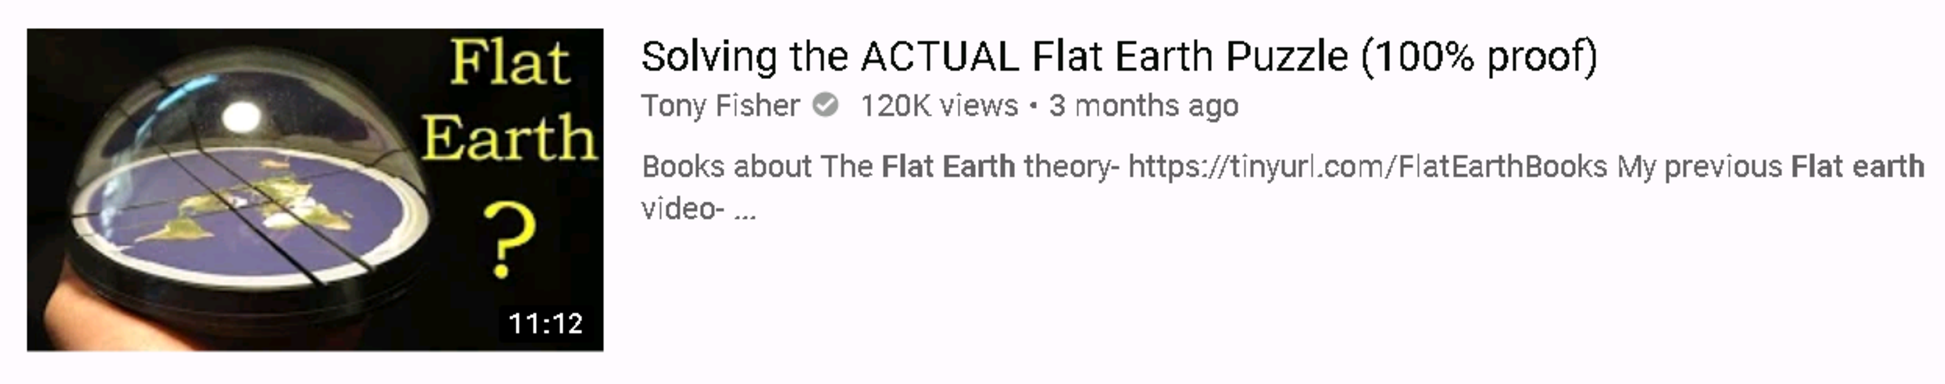
\includegraphics[scale=0.3]{Figures/Flat_earth.pdf}
% 		\end{minipage}
% 	\end{figure}

	
% 	\begin{figure}
		
% 	\end{figure}
% 	\begin{figure}
		
% 	\end{figure}
% 	\begin{figure}
		
% 	\end{figure}
\end{frame}

%%%%%%%%%%%%%%%%%%%%%%%%%%%%%%%%%%%%%

\begin{frame} \frametitle{Problem Statement}
\begin{columns}
		\column{0.5\textwidth}
		Consequences of fake news
	\begin{itemize}
			\item Distrust in science
			\item Conspiracy theories
			\item Less accessing of medicine
		\end{itemize}
		
		\column{0.5\textwidth}
\begin{figure}
		
\includegraphics[scale=0.3,frame]{Figures/Distrust.pdf}
	\end{figure}
			\end{columns}
	\begin{figure}
		
\includegraphics[scale=0.3,frame]{Figures/Vaccines_nz.pdf}
	\end{figure}
	\begin{figure}
		
\includegraphics[scale=0.25,frame]{Figures/Vaccines_us.pdf}
	\end{figure}
\end{frame}

%%%%%%%%%%%%%%%%%%%%%%%%%%%%%%%%%%%%%

\begin{frame} \frametitle{Solution}
	\centering
	\Huge Bullshit-o-meter
	\begin{figure}
		
\includegraphics[scale=0.5]{Figures/Deja_moo.jpg}
	\end{figure}
\end{frame}

%%%%%%%%%%%%%%%%%%%%%%%%%%%%%%%%%%%%%

\begin{frame} \frametitle{Methods}
	Browser plug-in
	\begin{itemize}
	    \item Gives a measure of the reliability of the current web-page
	    \item Measure is currently based on number of citations to academic papers
	    \item Suggests links to layman-friendly, reliable sources
	\end{itemize}
	\begin{figure}
		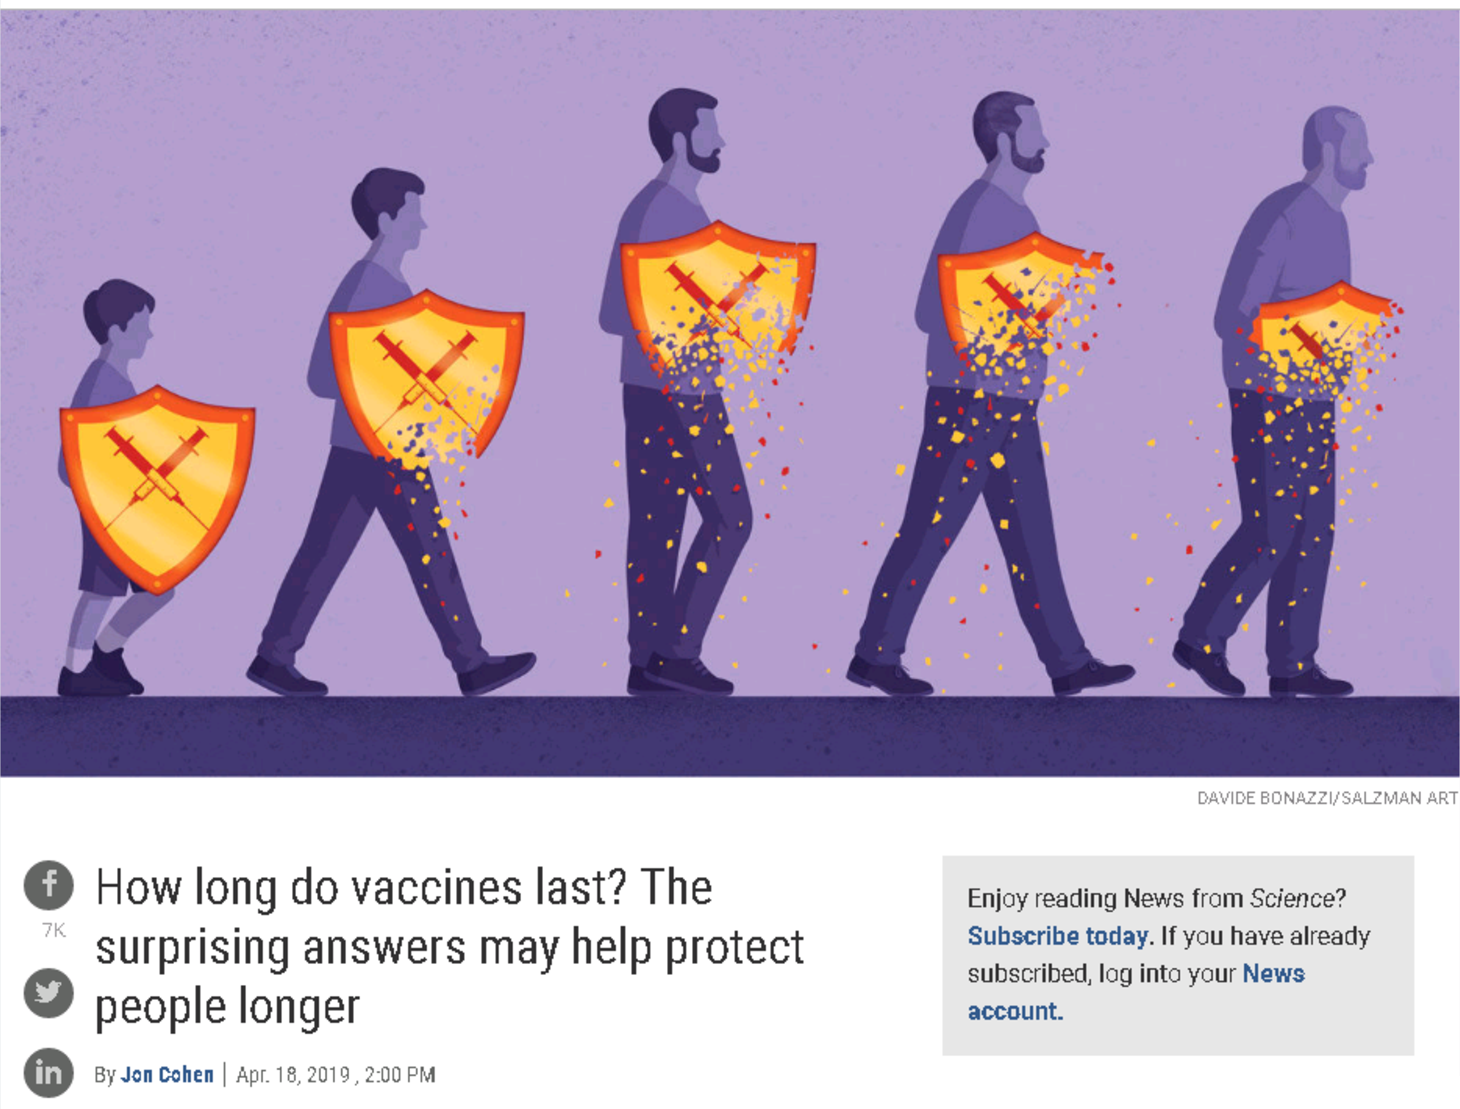
\includegraphics[scale=0.2]{Figures/webpage.pdf}
	\end{figure}
	\centering
	\href{https://www.sciencemag.org/news/2019/04/how-long-do-vaccines-last-surprising-answers-may-help-protect-people-longer?fbclid=IwAR2SRI_3p9j4aUWZDTyfPYf21PUJtjwojyErQg5rbUd3S-2MSFwjSxR9kfo}{Click here}
\end{frame}

%%%%%%%%%%%%%%%%%%%%%%%%%%%%%%%%%%%%%


\begin{frame} \frametitle{Scope}
	Browser plug-in
	\begin{itemize}
	\item Expand and refine reliability measure to include the rhetoric and phraseology of the pages content
	\end{itemize}
	Back-end user-curated open source repository
	\begin{itemize}
	    \item Expand reliable source repository to news articles and popular science materials. 
	    \item Enlist the help of institutions such as Universities of CRIs to expand and maintain the repository.
	\end{itemize}
	\centering
	\begin{tabular}{ c c }
		
\includegraphics[scale=0.1]{Figures/UC-Logo-3-2_3654775638524282877.jpg} & 
\includegraphics[scale=0.3]{Figures/mwlr-white-on-black.jpg}
	\end{tabular}
\end{frame}

%%%%%%%%%%%%%%%%%%%%%%%%%%%%%%%%%%%%%

\begin{frame}
	 \huge
	 \begin{center}
	 	Thank you for listening
	 \end{center} 
\end{frame}

\end{document}
